Il s'agit maintenant de d\'ecouvrir qu'est-ce qu'il y a dans mes donn\'ees. Comment montrer des choses apart de ce qui est gard\'e dans mon fichier. Par exemple dans le project de ce cours on montre le score obtenu. La visualisation des donn\'ees est tr\`es importante dans le monde de l'informatique d\'ecisionnelle (business intelligence) qui vise \`a donner les moyens pour collecter, consolider, mod\'eliser et restituer les donn\'ees d'une entreprise en vue d'offrir une aide \`a la d\'ecisiion et de permettre au d\'ecideur d'avoir une vue d'ensemble de l'activit\'e trait\'ee.

\subsection{Grammaire visuelles}

Ici on fait la visualisation en trois \'etapes:

1. \textbf{Placer les donn\'ees sur une image de base} de telle sorte que les propri\'t\'es visuelles de l'image refl\`etent les propri\'t'es abstraites des donn\'ees en particulier les relations entre donn\'ees. 

2. Cr\'eer une \textbf{grammaire visuelle} qui met en correspondance les variables des donn\'ees et les composantes graphiques. Si n\'ecessaire on cr\'ee une grammaire pour chaque dimension.

3. Mettre en \textbf{correspondance} un espace de n dimensions vers un espace de moindre dimensions par des m\'ethodes graphiques et des m\'ethodes statistiques.

\subsection{Principes de conception (Tufte)}

1. Choisir des unit\'es qui conservent du sens \`a travers les comparaisons. Exemple: wage minutes to by a hamburger in each country.

2. Choisir des unit\'es qui ont du sens pour le lecteur. Exemple: gross domestic product (GPD).

3. Choisir des intervalles pertinents. Exemple: a representation with big intervals can lead to not considering the whole information represented.

4. Evaluer les effets du choix des intervalles.

5. V\'erifier \textbf{l'int\'egrit\'e graphique}. Est-ce que l'importance visuelle correspond \`a la quantit\'e repr\'esent\'ee? Ici la perspective ou la r\'epresentation en 3D peuvent entra\^iner un pi\`ege.

6. Minimiser le "chart junk". Eviter les \'el\'ements qui n'apportent pas d'information et risquent de bruiter le message.

7. Optimiser le \textbf{"data ink ratio"}. Le data ink ratio c'est le quotient entre la quantit\'e de "ink" utilis\'ee to montrer le data entre la quantit\'e de "ink" utilis\'ee pour montrer le graphique. Elle devrait \^etre une magnitude \'elev\'ee outre on risque de utiliser trop d'\'elements graphiques pour r\'epresenter le data. Un donn\'ee peut s'identifier parce que si on l'efface, on perd de l'information.

8. Utiliser les \textbf{"small multiple"}. Il s'agit d'une s\'erie de graphiques similaires qui utilisent la m\^eme \'echelle et axes et qui permettent de les comparer facilement.

9. Montrer les co-variations. On montre sur un m\^eme graphique les variations des magnitudes r\'elationn\`ees . Ce qui permet \`a l'oeil de cr\'eer la correlation.

10. Montrer le contexte. Contextualiser l'information pour pr\'eciser son contenu.

\subsection{Distorsions g\'eom\'etriques}

Il n'existe pas de visualisation objective. Visualiser c'est communiquer.

On rencontre fr\'equentement des distorsions des visualizations qui peuvent \^etre forc\'ees ou n\'ecessaires.  

Exemples des \textbf{distorsions forc\'ees}: la repr\'esentation du globe terrestre sur le plan d'une carte. La Winker triple projection essaye de minimiser les distortion en termes de distance, angles et surfaces. La repr\'esentation d'une pyramide sur un plan, par exemple la r\'epresentation d'une montagne comme les Diablerets.

Il y a des autres distortions g\'eom\'etriques qui peuvent \^etre n\'ecessaires pour bien r\'epresenter l'objet sous \'etude. Par exemple le diagramme des lignes de m\'etro doit int\'egrer diff\'erent zones avec \textbf{diff\'erentes densit\'es}. Pour bien faire cette distorsion on peut utiliser des outils comme des \'echelles non-lin\'eaires, l'effet loupe ou des modes interactifs. 

On peut rencontrer des occassions ou il faut "tricher" pour rendre visible ce qui n'est pas visible. Par exemple si on repr\'sente les salaires et les ages d'un groupe des personnes et on veut savoir combien des personnes nous sommes en train d'\'etudier on peut ajouter du \textbf{bruit al\'eatoire ou "jitter"} aux donn\'ees pour rendre tous les points visible. En faisant \c{c}a, la visualization est fausse par respect \`a un axe mais plus correcte par rapport \`a la nature des donn\'es.

Une autre distortion n\'ecessaire peut \^etre \textbf{l'utilization des \'echelles incompatibles}. Par exemple si on veut representer une ascension alpiniste il est important de remarque l'ascension vertical m\^eme s'il est n\'egligeable en comparaison avec l'\'echelle horizontal. Ainsi on fait une exag\'eration dans certaines magnitudes. Une mesure pour d\'eterminer le degr\'e de distortion est le \textbf{Lie factor}. Il est le quotient entre l'effet montr\'e dans le graphique et l'effect montr\'e dans le data. 

Quelques distortions peuvent \textbf{communiquer des id\'ees}. Une carte standard peut \^etre distortion\'e pour montrer des informations sur la population ou le PIB de chaque pays. Le nombre des inscrits dans les cours de l'EPFL peut \^etre represent\'e par pays selon le nombre d'inscrits ou en r\'elation avec le nombre d'utilisateurs d'Internet.

\subsection{Erreurs fr\'equents dans la conception ou interpr\'etation des visualisations}

\begin{itemize}
\item Les couleurs ne fournissent pas d'information.
\item \textbf{L'empilement des graphiques} n\'ecessite de calculer mentalement les comparaisons.
\item Les \textbf{valeurs extr\^emes} \'ecrasent l’information. Une solution est l'utilisation d'\'echelles non-lin\'eaires par exemple l'\'echelle logarithmique.
\item Le syst\'eme g\'en\`ere automatiquement une \'echelle inappropri\'ee qui emp\^eche de faire des comparaisons correctes.
\item \textbf{Ordre des donn\'ees non justifi\'e}. Le pattern visuel produit d\'epend davantage de l’ordre des donn\'ees que des donn\'ees elles-m\^emes.
\item Ordre des donn\'ees innapropri\'e.
\item Les \textbf{points connect\'es} par des traits ne sont pas r\'eellement des donn\'ees li\'ees les unes aux autres.
\item \textbf{Sensibilit\'e de la moyenne aux valeurs extr\^emes}. C'est pour \c{c}a qu'on fait les analyses de variance. Dans les repr\'esentations graphiques de donn\'ees statistiques, la \textbf{bo\^ite \`a moustaches} est un moyen rapide de figurer le profil essentiel d'une s\'erie statistique quantitative.
\item \textbf{Sensibilit\'e des courbes de tendance}.
\item \textbf{Intepr\'eter une corr\'elation comme un lien de causalit\'e}. La corr\'elation peut \^etre en r\'ealit\'e caus\'ee par l'existence d'une \textbf{variable cach\'ee}. Ainsi probablement s'endormir avec une seule chaussure n'est pas la cause de se r\'eveiller avec un mal de t\^ete mais la cause peut \^etre tr\`es bien la consommation d'alcool.
\item Les \textbf{acronymes rares} pour l'utilisateur augmentent sa charge cognitive.
\item Le "split attention effect" augmente la charge cognitive.
\end{itemize}

The \textbf{split-attention effect} is a learning effect inherent within some poorly designed instructional materials. It is apparent when the same modality (e.g. visual) is used for various types of information within the same display. To learn from these materials, learners must split their attention between these materials to understand and use the materials provided.

Les \textbf{visualisations dynamiques} font usage de des utiles particuliers: changement d'\'echelle spatiale (zoom, croll,...), changement d'\'echelle temporelle, changement d'\'echelle des variables, rotations 2D ou 3D, changement de variables, "mouse over" (events that happen when the mouse is over the element)...

\subsection{Exercises}

\begin{figure}[H]
\centering
\makebox[\textwidth][c]{
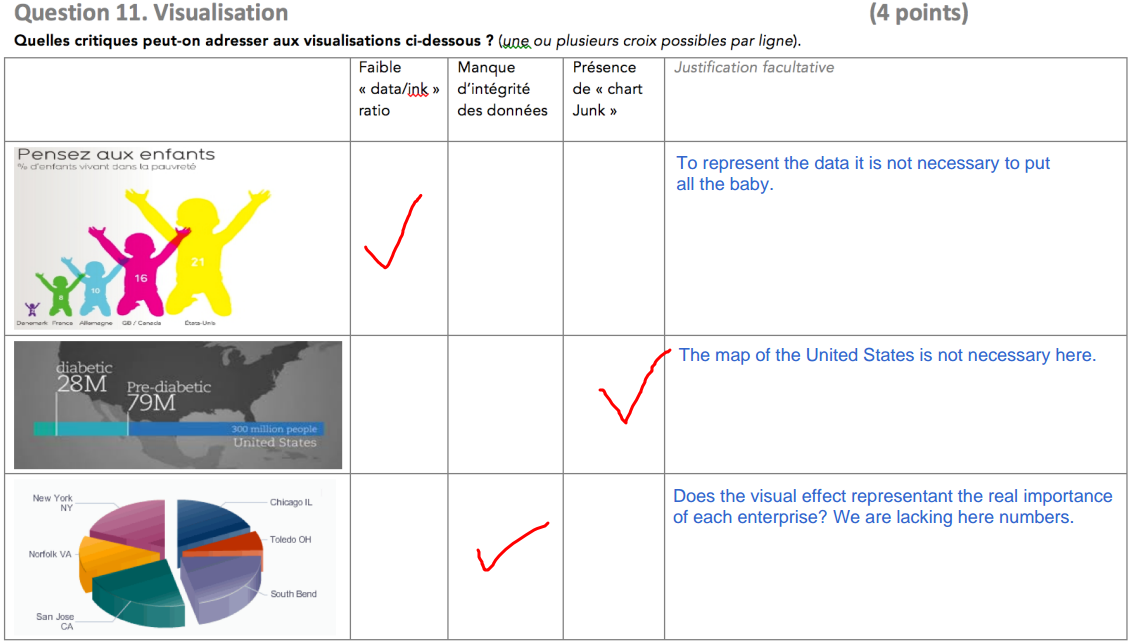
\includegraphics[scale=0.35]{./images/exercise1.png}
}
\end{figure}

\begin{exercise}
En rempla\c{c}ant une visualisation en 3D par un treillis de vues 2D, quels principes de visualisation des donn\'ees sont-ils mis en oeuvre? 
\end{exercise}

Eviter le split attention effet (pas correcte)

Eviter l'occlusion de certaines donn\'ees (correcte)

Eviter le lie factor (pas correcte)

Utiliser les small multiples (correcte)

Utiliser les distorsions (pas correcte)














